\documentclass[]{beamer}
\mode<presentation>{
  %% \usetheme[compress]{Berlin}
}
%% packages
\usepackage{zhspacing}
\zhspacing
\usepackage{graphics}
\usepackage{listings}
\lstset{basicstyle=\ttfamily\footnotesize}
\usepackage{tabularx}
\usepackage{booktabs}
%% meta info
\title{Clang ASTMatcher: Usage and Internals}
%\subtitle{An Introduction}
\author[SuXing~pysuxing@gmail.com]{SuXing}
\institute{TOW}
\date{\today}

%% slides
\begin{document}
\setlength{\parindent}{0pt}

\frame{\titlepage}

\frame{\tableofcontents}

\section{Using ASTMatcher}
\frame{\tableofcontents[currentsection]}

\begin{frame}
  \frametitle{AST matcher example}
  \lstinputlisting[language=C++]{listings/example.cpp}

  \pause
  Read from \alert{outside to inside}
\end{frame}

\begin{frame}
  \frametitle{AST matcher categories}
  AST matchers are categorized as
  \begin{itemize}
    \item Node Matchers\\
      Matchers that match a specific type of AST node
    \item Narrowing Matchers\\
      Matchers that match attributes on AST nodes
    \item Traversal Matchers\\
      Matchers that allow traversal between AST nodes
  \end{itemize}
\end{frame}

\begin{frame}
  \frametitle{Review: AST matche example}
  \lstinputlisting[language=C++]{listings/example-comment.cpp}

  \pause
  Note that matcher category \alert{usually} alternates between node matchers
  and narrowing or traversal matchers, but \alert{not necessarily}
\end{frame}

\begin{frame}
  \frametitle{More examples}
  \begin{itemize}
    \item<1-> switchStmt(forEachSwitchCase(caseStmt().bind("c")))
    \item<2-> recordDecl(hasMethod(hasName("func")))
    \item<3-> methodDecl(hasParameter(0, hasType(varDecl())))
  \end{itemize}
\end{frame}

\section{ASTMatcher Internals}
\frame{\tableofcontents[currentsection]}

\begin{frame}
  \frametitle{What are matchers are?}
  \begin{block}{Recall:}
    \centerline{recordDecl(hasMethod(hasName("func")))}
  \end{block}

  \pause
  \vspace{1em}
  These function-like objects, which we call \alert{matcher creators},
  includes
  \begin{itemize}
    \item ordinary functions
    \item functors, i.e. objects overloading operator ()
  \end{itemize}
\end{frame}

\begin{frame}
  \frametitle{What are matchers are? (cont.)}
  Matcher creators take \alert{Matcher} object(s) as parameters and return
  \alert{Matcher} object as result. 
  That is, by using matcher creators we got matchers of
  type \alert{Matcher<...>}
  \begin{figure}
    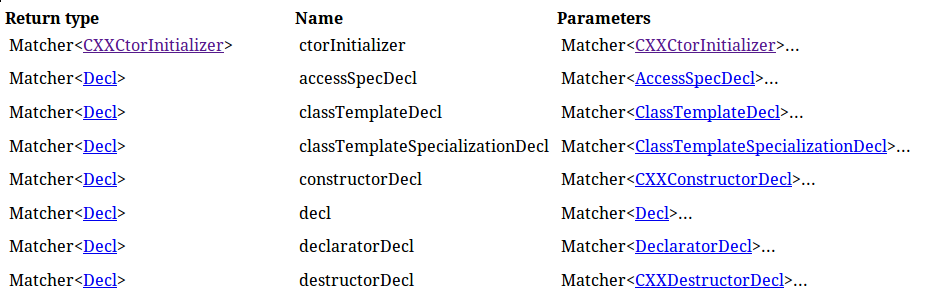
\includegraphics[width=\textwidth]{figures/matchers-prototype}
  \end{figure}
\end{frame}

\begin{frame}
  \frametitle{Star on stage: Matcher class template}
  \lstinputlisting[language=C++]{listings/Matcher.cpp}
  \pause
  A matcher of type Matcher<T> is intended to check if an AST node of type
  T satisfies some constraints. See \alert{matches} method's prototype above
\end{frame}

\begin{frame}
  \frametitle{Labor behind scenes: MatcherInterface class template}
  \lstinputlisting[language=C++]{listings/MatcherInterface.cpp}
  \pause
  Each Matcher<T> contains a MatcherInterface<T> member object and
  Matcher<T>::matches just forwards matching work to
  MatcherInterface<T>::matches.
\end{frame}

\begin{frame}
  \frametitle{Contradiction: usability of matcher creators}
  \begin{block}{prototype of a matcher creator}
    \centerline{Matcher<Result> SomeMatcherCreator(Matcher<Parameter>)}
  \end{block}
  \pause\vspace{1em}
  Here lies a contradiction:
  \begin{itemize}
    \item Matcher<Parameter> should work on any nodes satisfying
      Matcher<Result>, which means class Result must derive from
      Parameter \hfill \alert{--- C1}
    \item On the other hand, we want Matcher<Result> to work on all
      AST nodes withoud dynamic type dispatching, which requires
      Result to be root of AST node type hierarchies
      \hfill \alert{--- C2}
  \end{itemize}
\end{frame}

\begin{frame}
  \frametitle{Solve the contradiction: reverse type hierarchies}
  %%   \begin{block}{Recall:}
  %%     Clang AST contains a large number of node types,
  %%     forming class hierarchies rooted at several node
  %%     types (Decl, Stmt, ...)
  %%   \end{block}
  \begin{itemize}
    \item We make Result one of the roots, thus satisfying \alert{C2}
    \item We make Matcher<Result> implicitly convertable
    to Matcher<Parameter> providing that Parameter inherits from Result,
    thus satisfying \alert{C1}
  \end{itemize}
  \begin{figure}
    \includegraphics[width=.5\textwidth]{figures/hierachy}
  \end{figure}
  \pause
  We call this disign of Matcher<T> \alert{reverse hierarchies} because
  the implicit convertion from Matcher<Result> to Matcher<Parameter> is
  like a down-cast in normal type hierarchy.
\end{frame}

\begin{frame}
  \frametitle{Solve the contradiction: reverse type hierarchies (cont.)}
  \lstinputlisting[language=C++]{listings/MatcherCtor.cpp}
  \pause
  Matcher<T> has a template constructor, enabling implicit convertion
  from Matcher<From> if From is base class of T.

  \pause\vspace{1em}
  \alert{What's ImplicitCastMatcher?}
\end{frame}

\begin{frame}
  \frametitle{Solve the contradiction: reverse type hierarchies (cont.)}
  \lstinputlisting[language=C++]{listings/ImplicitCastMatcher.cpp}

  \pause
  \includegraphics[width=\textwidth]{figures/forward}

  ImplicitCastMatcher<Base> is a middle layer between Matcher<From> and
  Matcher<T>
\end{frame}

\begin{frame}
  \frametitle{All in one picture}
  \begin{figure}
    \includegraphics[width=\textwidth]{figures/allinone}
  \end{figure}
  \centerline{OutterMatcherCreator(InnerMatcherCreator())}
\end{frame}

\section{Writting AST Matchers}
\frame{\tableofcontents[currentsection]}

\begin{frame}
  \frametitle{AST Matcher components}
  Generally, a matcher is made up of two parts:
  \begin{itemize}
    \item A MatcherInterface implementation (labor)\\
      Overwritting the \alert{matches} method
    \item A matcher creator returning Matcher object (star)\\
  \end{itemize}
\end{frame}

\begin{frame}
  \frametitle{Using ASTMatcher Macros}
  ASTMatcher library provides some macros to simplify coding labor
  \begin{itemize}
    \item AST\_MATCHER
    \item AST\_MATCHER\_P
    \item AST\_MATCHER\_P2
    \item AST\_MATCHER\_P\_OVERLOAD
    \item AST\_MATCHER\_P2\_OVERLOAD
    \item ... (more complicate)
  \end{itemize}
\end{frame}

\begin{frame}
  \frametitle{An example: find small code blocks}
  \lstinputlisting[language=C++]{listings/smallblock.cpp}
  This will define a function \alert{statementCountLessThan}
  taking an \alert{unsigned} parameter and returning an 
  Matcher<\alert{CompoundStmt}> object whose matches method 
  will match all \alert{CompoundStmt} nodes with less than \alert{N}
  child statments in it.
\end{frame}

\section{Summary}
\frame{\tableofcontents[currentsection]}
\begin{frame}
  \frametitle{Summary}
  \begin{itemize}
    \item Using ASTMatcher\\
      Start from Node matchers, alternately use Node matchers and Narrowing
      or Traversal matchers.
    \item ASTMatcher Internals\\
      The Matcher class template and its reverse hierarchy design.
      Fairly tricky.
    \item Writting ASTMatchers\\
      Use ASTMatcher Macros, and knowledge of ASTMatcher internals helps
      a lot
  \end{itemize}
  \pause
  \alert{Only tip of the iceberg is touched!}
\end{frame}

\begin{frame}
  \frametitle{References}
  \begin{itemize}
    \item http://clang.llvm.org/docs/LibASTMatchersReference.html
    \item Source code
      \begin{itemize}
        \item \alert{clang/ASTMatchers/ASTMatchersInternal.h}
        \item clang/ASTMatchers/ASTMatchersMacros.h
        \item clang/ASTMatchers/ASTMatchers.h
      \end{itemize}
  \end{itemize}
\end{frame}

\frame{\centerline{\Huge Q\&A}}

\end{document}
